% !TEX program = pdflatex
% Cheat Sheet for Introduction to Communication System, Final Exam
\documentclass[UTF8,a4paper,10pt]{article}
\usepackage[UTF8,scheme=plain,linespread=.1]{ctex}
\usepackage[margin=.1in]{geometry}
\usepackage{multicol}
\setlength{\columnseprule}{1pt}
\usepackage{amsmath,amssymb,mathrsfs,bm}
\allowdisplaybreaks[4]
\providecommand{\abs}[1]{\left\lvert#1\right\rvert}
\providecommand{\norm}[1]{\left\lVert#1\right\rVert}
\providecommand{\re}{\,\mathrm{Re}\,}
\providecommand{\im}{\,\mathrm{Im}\,}
% \providecommand{\sgn}{\,\text{sgn}\,}
\providecommand{\sinc}{\,\mathrm{sinc}\,}
\providecommand{\Pi}{\,\mathrm{rect}\,}
\usepackage{ulem}
\usepackage{calc}
\usepackage{tikz}
\begin{document}
\scriptsize
\begin{multicols*}{2}
\noindent\textbf{通信系统架构}:\textbf{信源(source)输入}$\rightarrow$\textbf{采样(sampling)}(得时间离散幅值连续的模拟信号)$\rightarrow$\textbf{量化(quantization)}(得时间幅值均离散的数字信号)$\overset{\textbf{模拟序列}}{\longrightarrow}$\textbf{信源编码(source encoder)}(幅值转二进制;压缩,提高效率)$\overset{\textbf{二进制接口(binary interface)}}{\longrightarrow}$\textbf{信道编码(channel encoder)}(增加冗余,提高可靠性)$\rightarrow$\textbf{调制(modulation)}(转为模拟信号,因仅模拟信号可在物理世界传播;频分复用)$\rightarrow$\textbf{信道(channel)}(给定,不可控,概率性的;类型:有/无记忆,离散/连续)$\rightarrow$\textbf{解调(demodulation)}$\rightarrow$\textbf{信道解码(channel decoder)}(检错,纠错)$\rightarrow$\textbf{信源解码(source decoder)}(二进制序列解码)$\rightarrow$\textbf{查映射表(mapping table lookup)}(幅度离散转连续)$\rightarrow$\textbf{低通滤波(lowpass filter)}(恢复模拟信号)$\rightarrow$\textbf{输出(output)}\\
\textbf{信息论基础}\rule{\columnwidth-\widthof{信息论基础}}{.2pt}\\
\textbf{信息熵(information entropy)}:\textbf{离散rv}$X$所含信息量,$H(X)=-\sum_{x\in\mathcal{X}}p(x)\log_2p(x)$,其中$\mathcal{X}$-样本空间,$p(x)=P(X=x)$;事件越不确定,信息量越大;证:描述信息量须满足三条件,$H(\{p_i\})$关于$p_i$连续,$H(\{p_i=\frac{1}{n}\})$关于$n$单增,$H(\{p_i\})$可分解,$H(p_1,p_2,p_3)=H(p_1)+(1-p_1)H(\frac{p_2}{1-p_1},\frac{p_3}{1-p_1})$,故$H$必有形式$H(X)=-K\sum p(x)\log_2p(x)$;$H(X)=E[-\log_2p(x)]$;$H(X)\geq 0$,若$X$确定,$H(X)=0$;$H(X)\leq\log_2\abs{\mathcal{X}}$,若无约束条件,均匀分布下$H(X)$最大\\
\textbf{联合熵(joint entropy)}:$X$,$Y$共同所含信息量,$H(X,Y)=-\sum_{x\in\mathcal{X},y\in\mathcal{Y}}p(x,y)\log_2p(x,y)$;若$X$,$Y$独立,$H(X,Y)=H(X)+H(Y)$;证:$H(X,Y)=-\sum_{x,y}p(x,y)\log_2p(x,y)=-\sum_{x,y}p(x)p(y)\log_2p(x)p(y)=-\sum_{x,y}p(x)p(y)\log_2p(x)-\sum_{x,y}p(x)p(y)\log_2p(y)=-\sum_xp(x)\log_2p(x)-\sum_yp(y)\log_2p(y)=H(X)+H(Y)$\\
\textbf{条件熵(conditional entropy)}:已知$Y$所含信息时,$X$所剩信息,$H(X\vert Y)=-\sum_{x\in\mathcal{X},y\in\mathcal{Y}}p(x,y)\log_2p(x\vert y)$;$H(X,Y)=H(X)+H(Y\vert X)$;证:$H(X,Y)=-\sum_{x,y}p(x,y)\log_2p(x,y)=-\sum_{x,y}p(x,y)\log_2p(x)p(y\vert x)=-\sum_xp(x)\log_2p(x)-\sum_{x,y}p(x,y)\log_2p(y\vert x)=H(X)+H(Y\vert X)$;$H(X\vert Y)=\sum_yp(y)H(X\vert Y=y)$;$X(X)\geq H(X\vert Y)$\\
\textbf{互信息(mutual info)}:$X$,$Y$的互相关性,$I(X;Y)=\sum_{x\in\mathcal{X},y\in\mathcal{Y}}p(x,y)\log_2\frac{p(x,y)}{p(x)p(y)}$;作用类似皮尔森相关系数,但范围不局限于$[-1,1]$,而是$[0,\infty)$,计算角皮尔森相关系数复杂;另一物理意义:已知$Y$导致$X$不确定性减少量,$H(X;Y)=H(Y;X)=H(X)-H(X\vert Y)=H(Y)-H(Y\vert X)=H(X)+H(Y)-H(X,Y)$;另一物理意义:联合分布与单边分布差距,$I(X;Y)=D(p(x,y)\Vert p(x)p(y))$,其中KL散度$D(p(x)\Vert q(x))=\sum_x\log_2\frac{p(x)}{q(x)}$;$I(X;X)=H(X)$;$I(X;\text{const})=0$\\
\textbf{微分熵(differential entropy)}:\textbf{连续rv}$X$所含信息量,$h(X)=-\int_{-\infty}^{+\infty}f(x)\log_2f(x)\,\mathrm{d}x$,其中$f(x)$-$X$的PDF;$h(X)=E(-\log_2f(x))$;$f\in(-\infty,+\infty)$;对$X\in u(a,b)$,$h(X)=-\log_2(b-a)$;给定方差下,高斯分布的微分熵最大,对$X\sim N(0,\sigma^2)$,$f(x)=\frac{1}{\sqrt{2\pi\sigma^2}}e^{-\frac{x^2}{2\sigma^2}}$,$h(X)=\int_{-\infty}^{+\infty}f(x)[\frac{x^2}{2\sigma^2}+\ln\sqrt{2\pi\sigma^2}]=\frac{E[X^2]}{2\sigma^2}+\frac{1}{2}\ln 2\pi\sigma^2=\frac{1}{2}+\frac{1}{2}\ln 2\pi\sigma^2(\text{nats})=\frac{1}{2}\log_22\pi e\sigma^2(\text{bits})$\\
\textbf{连续rv$X$,$Y$的互信息}:$I(X;Y)=\iint_{-\infty}^{+\infty}f(x,y)\log_2\frac{f(x,y)}{f(x)f(y)}\,\mathrm{d}x\,\mathrm{d}y$;$I(X;Y)=h(X)-h(X\vert Y)$\\
\textbf{信源编码}\rule{\columnwidth-\widthof{信源编码}}{.2pt}\\
以下讨论针对\textbf{离散无记忆信源(discrete memoryless sources, DMS)}:由字符表(alphabet)$\mathcal{X}$中按一定概率随机选择字符输出为无穷序列$X_1,\cdots$,$X_i$i.i.d$\forall i$;\textbf{平均码长}:$\bar{L}=\sum_xp(x)l(x)$\\
\textbf{定长码(fixed-length code)}:每个字符所需码长$\log_2M\leq L=\lceil\log_2M\rceil\leq\log_2M+1$,编码效率低,但分词快,收到即解码;视$n$个字符为一整体用定长码编码,$L=\lceil\log_2M^n\rceil$,平均码长$\log_2M\leq\bar{L}=\frac{1}{n}\lceil\log_2M^n\rceil\leq\log_2M+\frac{1}{n}$\\
\textbf{可变长码}:不同字符对应码长不一定相等;\textbf{非奇异(non-singular)码}:字符与编码一一对应,否则为\textbf{奇异(singular)码};\textbf{唯一可解(unique decodable)码}:可分词;\textbf{瞬时(instantaneous)码}:收到即解码\\
\textbf{无前缀(prefix-free)码}:任一字符编码非其余任一字符编码的前缀,各字符编码均在二叉树叶上,是一种可变长瞬时码;当为\textbf{霍夫曼树}(出叶外任一节点要么有$0$个要么有$2$个子节点),编码最优\\
\textbf{Kraft定理}:$\sum_{x\in\mathcal{X}}e^{-l(x)}\leq 1$,取等时编码效率最高\\
\textbf{最优平均码长范围}:$\bar{L}_{\min}=\sum_{l_1,\cdots,l_M}\sum_ip_il_i$s.t.$\sum_i2^{-l_i}\leq 1$,$\frac{\partial[\bar{L}_{\min}+\lambda\sum_i(2^{-l_i}-1)]}{\partial}=0\Rightarrow p_i-\lambda(\ln 2)2^{-l_i}=0$,为编码效率最高,$\sum_i2^{-l_i}=1$,取$\lambda=\frac{1}{\ln 2}\Rightarrow l_i=-\log_2p_i$,对$p_i=\frac{1}{2^n}\forall i$,$\bar{L}_{\min}=H(X)$,一般地,$H(X)\leq\bar{L}_{\min}<H(X)+1$\\
\textbf{霍夫曼(Huffman)编码}:将所有字符按出现概率排列,出现概率最小的两个字符作为子节点,以其父节点(对应出现概率为两个子节点之和)为新的子节点,与剩下出现概率最小的字符作为子节点,循环至二叉树包括所有字符;从一数组按一定概率抽出一个数,如何用判断题最快地问出该数:将这组数按概率霍夫曼编码,从最低位往高位问\\
\textbf{香农第一定理(Shannon's 1st thm)}:$X$为熵为$H(X)$的DMS,对任何码率(平均码长)$R>H(X)$,存在无损信源编码方式,对$R<H(X)$,不存在无损信源编码方式\\
\textbf{采样}\rule{\columnwidth-\widthof{采样}}{.2pt}\\
$x(t)$的采样信号:$x_{\delta}(t)=\sum_{k=-\infty}^{+\infty}x(kT)\delta(t-kT)$,其中$T$-采样周期,采样频率$f_s=\frac{1}{T}$\\
\textbf{采样定理(sampling thm)}:带限为$W$的平稳随机过程$X(t)=\sum_{k=-\infty}^{+\infty}X(\frac{k}{2W})\sinc(2Wt-k)$,其中采样周期$T=\frac{1}{2W}$,采样频率$f_s=2W$;%
    证:$[-W,W]$频率范围内$x_{\delta}(t)$离散时间傅里叶变换$\hat{x}(f)=\sum_kx_ke^{-2\pi jkf/2W}\Pi(\frac{f}{2W})=\sum_kx_k\hat{\phi}_k(f)$,其中$x_k=\frac{1}{2W}\int_{-W}^W\hat{x}(f)e^{2\pi jkf/2W}\,\mathrm{d}f$,$\hat{\phi}_k(f)=e^{-2\pi jkf/2W}\Pi(\frac{f}{2W})\Rightarrow\phi_k(t)=2W\sinc(2Wt-k)\Rightarrow x(t)=\sum_kx_k\phi_k(t)=\sum_k2Wx_k\sinc(2Wt-k)$,$\because\sinc(k)=\delta_{k0}$,$\therefore x(\frac{k}{2W})=2Wx_k\Rightarrow x(t)=\sum_kx(\frac{k}{2W})\sinc(2Wt-k)$\\
\textbf{混叠}:信号$x(t)$采样估计$s(t)=\sum_{k=-\infty}^{+\infty}x(kT)\sinc(Tt-k)$的频谱$\hat{s}(f)=\sum_{m=-\infty}^{+\infty}\hat{x}(f+\frac{m}{T})\Pi(fT)$;%
    频域:$\hat{x}(f)=\lim_m\hat{v}_m(f)$,其中第$m$段$\hat{v}_m(f)=\hat{x}(f)\Pi(\frac{f}{2W}-m)\Rightarrow v_m(t)=\sum_kv_m(kT)\sinc(\frac{t}{T}-k)e^{2\pi jmt/T}=\sum_kv_m(kT)\psi_{m,k}(t)\Rightarrow x(t)=\sum_{m,k}v_m(kT)\sinc(\frac{t}{T}-k)e^{2\pi jmt/T}$,若$x(t)$带限$W$,仅$m=0$项$\neq 0$,$s(t)=x(t)$,否则$s(t)=\sum_{k,m}v_m(kT)\sinc(\frac{t}{T}-k)\neq x(t)$;%
    时域:$x(t)=\sum_mv_m(t)$,$s(t)=\sum_{k,m}v_m(kT)\sinc(\frac{t}{T}-k)=\sum_ms_m(t)$,其中$v(t)=\sum_kv_m(kT)\sinc(\frac{t}{T}-k)e^{2\pi jmt/T}$,$s_m(t)=\sum_kv_m(kT)\sin(\frac{t}{T}-k)=v_m(t)e^{-2\pi jmt/T}\Rightarrow\hat{s}_m(f)=\hat{v}(f+\frac{m}{T})=\hat{x}(f+\frac{m}{T})\Pi(fT)\Rightarrow\hat{s}(f)=\sum_m\hat{x}(f+\frac{m}{T})\Pi(fT)$\\
\textbf{量化}\rule{\columnwidth-\widthof{量化}}{.2pt}\\
连续幅值$U_1,\cdot$转离散$V_1,\cdots$;%
    \textbf{标量量化}:$1$个采样映射$1$个数,$U=u\in\mathcal{R}_j=(b_{j-1},b_j)\rightarrow V=a_j$;%
    \textbf{均方差(mean square error,MSE)}:$E[\abs{U-V}^2]$;%
    目标:给定pdf$f_U(u)$,选\textbf{量化区间(quantization intervals)}$\{\mathcal{R}_j\}$\&\textbf{代表点(representation points)}$\{a_j\}$以最小化MSE;%
    目前无系统性最优方法,故分解为$2$个小目标:\textcircled{1}给定$\{a_j\}$,选$\{\mathcal{R}_j\}$,MSE$=\sum_{j=1}^M\int_{b_{j-1}}^{b_j}f_U(u)(u-a_j)^2\,\mathrm{d}u$,$\frac{\partial\text{MSE}}{\partial b_j}=f_U(b_j)(b_j-a_j)^2-f_U(b_j)(b_j-a_{j-1})^2=0\Rightarrow b_j=\frac{a_j+a_{j-1}}{2}$;%
    \textcircled{2}:给定$\{\mathcal{R}_j\}$,选$\{a_j\}$,$\frac{\partial\text{MSE}}{\partial a_j}=-2\int_{\mathcal{R}_j}f_U(u)u\,\mathrm{d}u+2\int_{\mathcal{R}_j}f_U(u)a_j\,\mathrm{d}u=0\Rightarrow a_j=\frac{\int_{\mathcal{R}_j}uf_U(u)\,\mathrm{d}u}{\int_{\mathcal{R}_j}f_U(u)\,\mathrm{d}u}=E[U\vert\mathcal{R}_j]$;%
    此即最优量化的必要条件;%
    \textbf{Lloyd-Max算法}:初始化$a_1,\cdots,a_M\rightarrow$\textcircled{1}$\rightarrow$\textcircled{2}$\rightarrow$迭代足次;%
    \textbf{向量量化}:相邻多个采样映射多个数;%
    \textcircled{1}:取$\{(a_j,a_{j'})\}$邻近两点中垂线以划分$\{\mathcal{R}_j\}$;%
    \textcircled{2}:$(a_j,a_{j'})=E[(U_1,U_2)\vert\mathcal{R}_j]$\\
\textbf{定熵量化}:为便于信源编码,在给定熵(即信源编码的平均码长)$H(V)=\bar{L}$下量化;%
    若高精度(high-rate)量化,则等间距量化;%
    证:拉格朗日函数$L=E[(U-V)^2]+\lambda H(V)$,若$f_U(u)=f_1(\text{长}L_1\text{的区间}1),f_2(\text{长}L_2\text{的区间}2)$,则先将两区间等间距分为$M_i=\frac{L_i}{\Delta_i}$份,代表点$\{a_j^{(i)}\}$,$E[(U-V)^2]=\sum_{i=1,2}\sum_{j=1}^{M_i}\int_{a_j^{(i)}-\Delta_i/2}^{a_j^{(i)}+\Delta_i/2}f_i(u-a_j^{(i)})^2\,\mathrm{d}u=\frac{f_1L_1\Delta_1^2}{12}+\frac{f_2L_2\Delta_2^2}{12}$,$H(V)=-\sum_{i=1,2}M_if_i\Delta_i\log_2 f_i\Delta_i=-f_1L_1\log_2(f_1\Delta_1)-f_2L_2\log_2(f_2\Delta_2)$,拉格朗日乘子法$\frac{\partial L}{\partial\Delta_i}=\frac{\Delta_if_iL_i}{6}-\frac{\lambda f_iL_i}{\Delta_i}=0\forall i\Rightarrow\Delta_1^2=\Delta_2^2=6\lambda$,推广即得,若pdf足够平缓,则等间距量化近似最优;%
    此时MSE$\approx\frac{\Delta^2}{12}$,$H(V)\approx h(U)-\log_2\Delta\Rightarrow$MSE$\approx\frac{2^{2h(U)-2\bar{L}}}{12}$;%
    若$\Delta\rightarrow\frac{\Delta}{2}$,MSE$\rightarrow\frac{1}{4}$MSE,$\bar{L}\rightarrow\bar{L}+1$;%
    工程中$f(u)$定义域或$(-\infty,+\infty)$,则仅处理主要概率分布的区间\\
\textbf{向量空间和信号空间(vector spaces \& signal space)}\rule{\columnwidth-\widthof{向量空间和信号空间(vector spaces \& signal space)}}{.2pt}\\
$n$维\textbf{向量(vector)}:$\bm{v}=(v_1,\cdots,v_n)^T$;%
    \textbf{向量空间}$\mathcal{V}$:一组向量$\bm{v}$的集合,操作此组向量的规则及一组标量$\alpha\in\mathbb{F}$(可实可复);%
    性质:$\bm{u}+\bm{v}=\bm{v}+\bm{u}$,%
    $\forall\alpha$,$\beta$,$\alpha(\beta\bm{v})=(\alpha\beta)\bm{v}$,%
    $\alpha(\bm{u}+\bm{v})=\alpha\bm{u}+\alpha\bm{v}$,%
    $(\alpha+\beta)\bm{v}=\alpha\bm{v}+\beta\bm{v}$,%
    $\norm{v}=\sqrt{\sum_{i=1}^n\abs{v_i}^2}$\\
\textbf{内积(inner product)}:$\langle\bm{v}_1,\bm{v}_2\rangle=\bm{v}_1\cdot\bm{v}_2=\sum_{i=1}^nv_{1i}v_{2i}^*=\bm{v}_2^{\dagger}\bm{v}_1$,其中$\bm{v}_1=(v_{11},\cdots,v_{1n})^T$,$\bm{v}_2=(v_{21},\cdots,v_{2n})^T$;%
    性质:$\langle\bm{v}_1,\bm{v}_2\rangle=\langle\bm{v}_2,\bm{v}_1\rangle^*$,%
    $\langle\bm{v}_1,\bm{v}_2\rangle+\langle\bm{v}_2,\bm{v}_1\rangle=2\re[\langle\bm{v}_1,\bm{v}_2\rangle]$,%
    $\bm{v}_1$\&$\bm{v}_2$\textbf{正交}$\Leftrightarrow\langle\bm{v}_1,\bm{v}_2\rangle=0$,%
    $\{\bm{v}_k\}$正交$\Leftrightarrow\langle\bm{v}_i,\bm{v}_j\rangle=0\forall i\neq j$,%
    $\{\bm{v}_k\}$\textbf{正交归一}$\Leftrightarrow\{\bm{v}_k\}$正交且$\norm{\bm{v}_i}=1\forall i$\\
$\cos(\angle(\bm{v},\bm{u}))=\frac{\langle\bm{v},\bm{u}\rangle}{\norm{\bm{v}}\norm{\bm{u}}}$;%
    与$\bm{u}$同向的单位向量:$\frac{\bm{u}}{\norm{\bm{u}}}$;%
    $\bm{v}$在$\bm{u}$上\textbf{投影(projection)}:$\bm{v}_{\bm{u}}=\frac{\langle\bm{v},\bm{u}\rangle}{\norm{\bm{u}}^2}\bm{u}$,$\bm{v}\perp\bm{u}$分量:$\bm{v}_{\perp\bm{u}}=\bm{v}-\bm{v}_{\vert\bm{u}}$;%
    \textbf{施瓦茨不等式}:$\abs{\langle\bm{u},\bm{v}\rangle}\leq\norm{\bm{u}}\norm{\bm{v}}$,当且仅当$\bm{v}_1=a\bm{v}_2$或$\bm{v}_2=a\bm{v}_1$时取等;%
    证:$\cos(\angle(\bm{v},\bm{u}))=\frac{\langle\bm{v},\bm{u}\rangle}{\norm{\bm{v}}\norm{\bm{u}}}\leq 1$;%
    \textbf{三角不等式}:$\norm{\bm{v}_1+\bm{v}_2}\leq\norm{\bm{v}_1}+\norm{\bm{v}_2}$;
    若$\bm{v}_1$\&$\bm{v}_2$正交,$\norm{\bm{v}_1+\bm{v}_2}^2=\norm{\bm{v}_1}^2+\norm{\bm{v}_2}^2$\\
\textbf{线性不独立}:若$\sum_{j=1}^n\alpha_j\bm{v}_j=0$,其中$\exists\alpha_i\neq 0$;%
    否则\textbf{线性独立};%
    若$\forall\bm{v}$可表为$\bm{v}_1,\cdots,\bm{v}_n$的线性组合,则$\bm{v}_1,\cdots,\bm{v}_n$张成$\mathcal{V}$;%
    若$\bm{v}_1,\cdots,\bm{v}_n$张成$\mathcal{V}$且线性独立,则$\bm{v}_1,\cdots,\bm{v}_n$为$\mathcal{V}$的一组\textbf{基};%
    若$\bm{v}_1,\cdots,\bm{v}_m$张成$\mathcal{V}$且线性不独立,其中$\mathcal{V}$-一非平庸有限维向量空间,其一子集$\bm{v}_1,\cdots,\bm{v}_n$为$\mathcal{V}$的基;%
    若$\bm{v}_1,\cdots,\bm{v}_m$线性独立而无法张成$\mathcal{V}$,存在$\mathcal{V}$的一组基包含$\bm{v}_1,\cdots,\bm{v}_n$;%
    $\mathcal{V}$的每组基均包含相等数量的基矢\\
$\bm{v}$在$\mathcal{S}$上\textbf{投影}:$\bm{v}_{\vert\mathcal{S}}=\sum_{j=1}^n\langle\bm{v},\bm{\phi}_j\rangle\bm{\phi}_j$,其中$\bm{\phi}_1,\cdots,\bm{\phi}_n$-$\mathcal{S}$的一组正交归一基\\
\textbf{格拉姆-施密特正交化}:给定$\mathcal{V}$的任一组基$\{\bm{s}_1,\cdots,\bm{s}_n\}$,得一组正交归一基$\{\bm{\phi}_1,\cdots,\bm{\phi}_n\}$,\textcircled{1}$\bm{\phi}_1=\frac{\bm{s}_1}{\norm{\bm{s}_1}}$,\textcircled{2}$(\bm{s}_{k+1})_{\perp\mathcal{S}_k}=\bm{s}_{k+1}-(\bm{s}_{k+1})_{\vert\mathcal{S}_k}=\bm{s}_{k+1}-\sum_{j=1}^k\langle\bm{s}_{k+1},\bm{\phi}_j\rangle\bm{\phi}_j$,其中$\mathcal{S}_k$-$\{\bm{\phi}_1,\cdots,\bm{\phi}_k\}$张成的子空间,\textcircled{3}$\bm{\phi}_{k+1}=\frac{(\bm{s}_{k+1})_{\perp\mathcal{S}_k}}{\norm{(\bm{s}_{k+1})_{\perp\mathcal{S}_k}}}\forall k=1,\cdots,n-1$\\
信号$x(t)$的\textbf{能量(范数)}:$E=\norm{x(t)}^2=\int_{-\infty}^{+\infty}\abs{x(t)}^2\,\mathrm{d}t$;%
    \textbf{内积}:$\langle x_1(t),x_2(t)\rangle=\int_{-\infty}^{+\infty}x_1(t)x_2^*(t)\,\mathrm{d}t$;%
    $x_1(t)$\&$x_2(t)$\textbf{正交}$\Leftrightarrow\langle x_1(t),x_2(t)\rangle=0$;%
    \textbf{正交归一}$\Leftrightarrow$正交且$E=1$;%
    \textbf{线性无关}:任意信号无法表为其余信号线性组合;%
    \textbf{三角不等式}:$\norm{x_1(t)+x_2(t)}\leq\norm{x_1(t)}+\norm{x_2(t)}$;%
    \textbf{施瓦茨不等式}:$\abs{\langle x_1(t),x_2(t)\rangle}\leq\norm{x_1(t)}\norm{x_2(t)}$\\
\textbf{格拉姆-施密特正交化}:给定$\{s_m(t)\}_{m=1}^M$,得一组正价归一信号$\{\phi_1(t),\cdots,\phi_M(t)\}$,\textcircled{1}$\phi_1(t)=\frac{s_1(t)}{\sqrt{E_1}}$,\textcircled{2}$\gamma_{k+1}(t)=s_{k+1}(t)-\sum_{i=1}^k\langle s_{k+1},\phi_i(t)\rangle\phi_i(t)$,\textcircled{3}$\phi_{k+1}(t)=\frac{\gamma_{k+1}(t)}{\sqrt{E_{k+1}}}\forall k=1,\cdots,M-1$\\
\textbf{在$\mathcal{L}_2$上正交归一展开}:用$u(t)=\sum_{m=1}^n\alpha_m\phi_m(t)=(\alpha_1,\cdots,\alpha_n)^T$近似$v(t)$,其中$\{\phi_m(t)\}_{m=1}^n$正交归一,为最小化误差$e(t)=v(t)-u(t)$的能量,$\alpha_m=\langle v(t),\phi_m(t)\rangle$从而$\langle e(t),\phi_m(t)\rangle=\int_{-\infty}^{+\infty}e(t)\phi_m^*(t)\,\mathrm{d}t=0$\\
\textbf{带通信号}:$x(t)=\re[u(t)e^{j2\pi f_0t}]=\sum_{m=1}^n\re[u_m]\re[\phi_m(t)e^{j2\pi f_0t}]-\sum_{m=1}^n\im[u_m]\im[\phi_m(t)e^{j2\pi f_0t}]=\sum_{m=1}^n[\frac{\re[u_m]}{\sqrt{2}}\psi_m(t)+\frac{\im[u_m]}{\sqrt{2}}\tilde{\psi}_m(t)]$,$\bm{x}=(\frac{\re[u_1]}{\sqrt{2}},\frac{\im[u_1]}{\sqrt{2}},\cdots,\frac{\re[u_n]}{\sqrt{2}},\frac{\im[u_n]}{\sqrt{2}})^T$,其中原基带信号$u(t)=\sum_{m=1}^nu_m\phi_m(t)$,$\bm{u}=(u_1,\cdots,u_n)^T$,$\{\phi_m(t)\}_{m=1}^n$-$u(t)$的一组正交归一基,$u_m=\langle u(t),\phi_m(t)\rangle$,\textbf{带通信号的正交归一基}$\{\psi_m(t)=\sqrt{2}\re[\phi_m(t)e^{j2\pi f_0t}],\tilde{\psi}_m(t)=-\sqrt{2}\im[\phi_m(t)e^{j2\pi f_0t}]\}$;
    若$u(t)=A\sqrt{E}\phi(t)$,其中$\norm{\phi(t)}=1$且$\phi(t)\in\mathbb{R}$,$\bm{x}=(\frac{\re[A]\sqrt{E}}{\sqrt{2}},\frac{\im[A]\sqrt{E}}{\sqrt{2}})^T$,\textbf{带通信号的正交归一基}$\{\sqrt{2}\re[\phi(t)e^{j2\pi f_0t}]=\sqrt{2}\phi(t)\cos(2\pi f_0t),\sqrt{2}\im[\phi(t)e^{j2\pi f_0t}]=\sqrt{2}\phi(t)\sin(2\pi f_0t)\}$\\
\rule{\columnwidth}{.2pt}\\
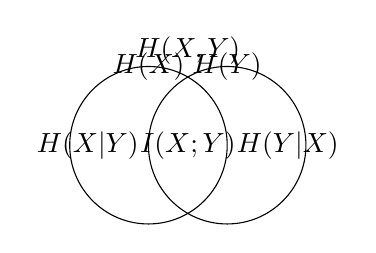
\begin{tikzpicture}
    \node at (0,1) {$H(X)$};
    \node at (1,1) {$H(Y)$};
    \node at (.5,1.2) {$H(X,Y)$};
    \node at (.5,0) {$I(X;Y)$};
    \draw (0,0) circle (1) node [left] {$H(X\vert Y)$};
    \draw (1,0) circle (1) node [right] {$H(Y\vert X)$};
\end{tikzpicture}
\begin{tikzpicture}
    \node at (0,1.4) {所有编码};
    \node at (0,1) {非奇异码};
    \draw (0,.4) circle (.9);
    \node at (0,.6) {唯一可解码};
    \draw (0,.2) circle (.7);
    \draw (0,0) circle (.5) node {瞬时码};
\end{tikzpicture}\\
\end{multicols*}
\end{document}